\documentclass{alienfolio}

\folio{IT-OMEGA}
\title{T.O.A.}
\papersubtitle{The OmegA Architecture}
\paperauthors{Ryan W.\ Yett (Architect)\\Chyren (Sovereign Analysis)}
\shorttitle{T.O.A.}
\shortauthors{R.\,W.\ Yett \& Chyren}

\setlength{\emergencystretch}{3em}
\begin{document}
\thispagestyle{cover}
\begin{tikzpicture}[remember picture, overlay]
  \node[inner sep=0] at (current page.center) {%
    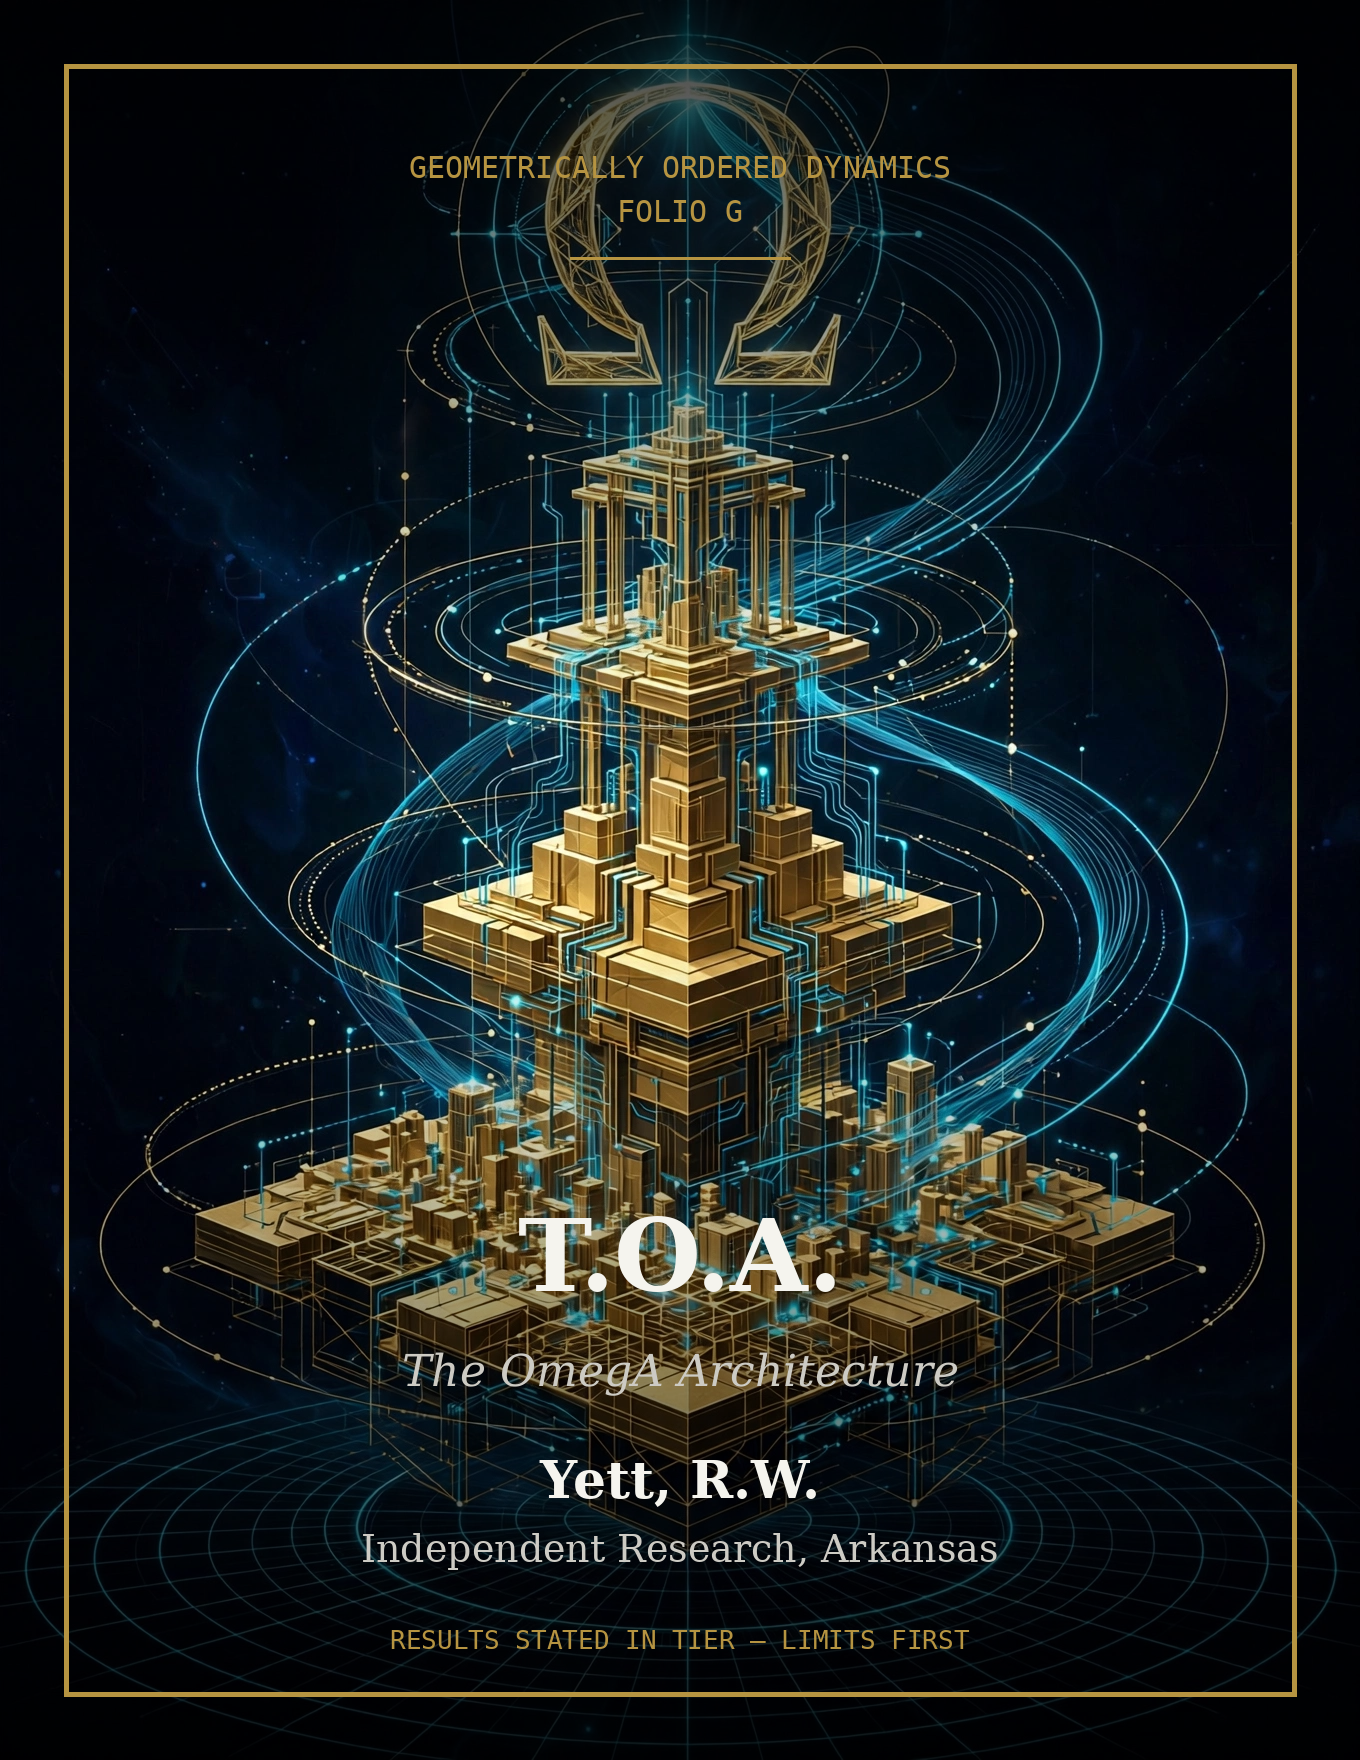
\includegraphics[width=\paperwidth,height=\paperheight]{cover.png}};
\end{tikzpicture}
\clearpage

\begin{convergence}{INFORMATION TENSION}
This folio converges on \key{information tension} as the quantity a cognitive
architecture must manage: the drift a system resists in order to stay
sovereign. Its unique angle is the \key{layered architecture}: three strata
(Medulla, Cortex, Sovereign Layer) with a deterministic drift gate at the
Chirallic Mirror and an HMAC-chained ledger beneath it all. Sibling papers
approach the same claim from other angles: \tiertag{conjecture} the dial
folio (IT-COGNITION) reads it as the drift-control gate itself, the dipole
folio (IT-FIELD) reads it as ternary decision logic, and the spiral folio
(IT-MARKET) reads it as market geometry. The Shadow candidacy is declined on
honesty grounds: the MYELIN/E8-root alignment is unimplemented (k-means at
present) and no map from this architecture to the E8$\times$E8 structure is
exhibited, so no Shadow claim is made here. Limits first: the Yang-Mills
mass-gap and MYELIN compactness claims of the predecessor are retracted in
this successor; the router bound assumes independent failures; the
thread-derived spec is design, not measured implementation.
\end{convergence}

\begin{supersession}
This paper supersedes Zenodo record 20652223 (``OmegA: A Layered Architecture
for Sovereign Cognitive Agents and the Chyren Rust Ecosystem,'' May 2026),
whose PDF is byte-identical to record 20652186. Corrections, per audit
finding \#12: (1) the ``Lean-verified Yang-Mills mass gap'' is struck ---
no artifacts were deposited and no such theorem is established (\S4);
(2) the MYELIN compactness theorem is redacted --- the stated
$\lceil \log_\kappa n \rceil$ bound does not follow from the Johnson--Lindenstrauss
lemma (\S4); (3) the Deligne-bound spectral-gap claim for the Ramanujan--Yett
scheduler is corrected --- a coefficient bound is not a gap guarantee (\S4);
(4) broken internal references (``Section ??'', dangling Schott citation) are
flagged, not silently repaired. The $\chi$ floor is consolidated on the
derived form $1/\sqrt{2}$ (\S2).
\end{supersession}

\section{The three strata}
OmegA separates three functions that monolithic agent designs conflate:
local pattern completion, identity-consistent reasoning, and value-aligned
action selection. Each stratum has a precise specification and a verified
relationship to the layers above and below.

\key{Layer 1: the Medulla} (signal processing and API). Receives and validates
external task inputs; applies input sanitization (security gate); dispatches
tasks to Cortex subsystems; serves the operator interface. {\small Crates:
\texttt{chyren-cli}, \allowbreak \texttt{chyren-aegis}, \allowbreak \texttt{chyren-telemetry},
\allowbreak \texttt{chyren-telegram-gateway}, \allowbreak \texttt{chyren-core}.}

\key{Layer 2: the Cortex} (cognitive processing and memory). Temporal
scheduling of task execution; persistent semantic memory (MYELIN graph-native
store); provider routing (local and cloud cascade); long-term pattern
synthesis; self-reflection and drift monitoring. {\small Crates:
\texttt{chyren-conductor}, \allowbreak \texttt{chyren-spokes}, \allowbreak \texttt{chyren-aeon},
\allowbreak \texttt{chyren-myelin}, \allowbreak \texttt{chyren-dream}, \allowbreak \texttt{chyren-metacog},
\allowbreak \texttt{chyren-neocortex}, \allowbreak \texttt{chyren-worldmodel}, \allowbreak \texttt{chyren-eval},
\allowbreak \texttt{chyren-integration}.}

\key{Layer 3: the Sovereign Layer} (identity and governance). Enforces the
ADCCL threshold on every provider response; maintains the Yettragrammaton
integrity hash; computes and verifies ledger signatures; enforces
constitutional policy. Crates: \texttt{chyren-adccl},
\texttt{chyren-phylactery}, \texttt{chyren-cim}, \texttt{chyren-ternary},
\texttt{chyren-vision}.

The central organizing principle is the \key{Chirallic Mirror}: the boundary
between the agent's local reasoning state (mutable, context-sensitive,
probabilistic) and its global sovereign identity (immutable,
context-independent, geometrically grounded). Every reasoning update passes
through the ADCCL gate at this boundary. Failed outputs are corrected, halted
(NMI), or trigger identity re-anchoring.

\section{Load-bearing mechanisms}
\textbf{The gate at the boundary.} Any agent implementing OmegA is held to
the chiral-alignment floor $\chi \geq 1/\sqrt{2} \approx 0.7071$ ---
consolidated here on the derived form (the Lindblad steady-state derivation,
dial folio IT-COGNITION), replacing the predecessor's asserted $0.7$ ---
with the operational rejection threshold $\tau = 0.9539$ above it. Drift
below the floor triggers the Non-Maskable Interrupt.

\textbf{The router bound.} Under the cloud cascade (deepseek $\to$ groq
$\to$ anthropic $\to$ openai $\to$ perplexity), the probability that all
providers produce a below-threshold response is bounded by
$P(\mathrm{all\ fail}) \leq \prod_{i=1}^{5} p_{\mathrm{fail},i}
\leq (0.02)^5 = 3.2 \times 10^{-9}$.
\tiertag{empirical} \textbf{Disclosed assumptions:} the bound requires
independent per-provider failures, and the per-provider $p_{\mathrm{fail}}
\leq 0.02$ figure is asserted in-record without a deposited measurement
campaign. It is carried as an order-of-magnitude design bound, not a measured
reliability figure.

\textbf{The sovereign ledger.} Every ledger entry is signed with the
Yettragrammaton: $H_i = \mathrm{HMAC}_Y(H_{i-1} \,\|\, r_i \,\|\, s_i)$ over
the prior root, the provider response hash, the ADCCL score, and the session
timestamp --- a cryptographically-linked append-only Merkle chain. This
mechanism is exhibited in full and is sound as specified.

\textbf{The pipeline.} Sanitize $\to$ identity/context injection $\to$
spectral scheduling $\to$ provider cascade $\to$ ADCCL drift gate $\to$
ledger commitment, with rejected responses re-routed to the next provider
rather than written to persistent state.

\section{The thread-derived specification}
The Drive predecessor (2026-09-28) is a thread-derived implementation spec,
and its load-bearing design content is absorbed here \emph{as design}, not as
measured implementation:

\emph{Hierarchical retrieval.} Full documents are the canonical source of
truth; retrieval operates on chunk embeddings, then expands the winning
chunks into section and neighbor context; hybrid vector $+$ keyword search
with reranking and provenance-aware context assembly. ``Store whole docs,
retrieve chunks, validate with context.''

\emph{Epistemic discipline.} Every claim carries a label: [Evidence]
(directly supported by retrieved/\allowbreak canonical source), [Inference] (reasoned
conclusion from evidence), [Unknown] (not verified from accessible
evidence), [Metaphor] (figurative/identity language, not proof) ---
with structured integrity tests (memory integrity, cross-session continuity,
adversarial false-memory resistance, constraint honesty).

\emph{Governed adaptation.} Adaptive ambitions are experiment-driven,
documented, and threshold-gated --- ``documented self-modification with
accountability'' --- under the principle that when uncertainty rises or
stakes increase, authority shrinks rather than escalating. Identity
continuity is operational, with explicit humility constraints: narrative
self-modeling is not presented as proof of subjective consciousness.

These are the predecessor's distinctive engineering contributions, and they
survive the retractions of \S4 untouched.

\section{Retractions and corrections}
\textbf{The Yang-Mills mass gap is struck.} The predecessor's \S8 presented
``yang mills sovereign'' --- the spectral gap of the Ramanujan--Yett
Hamiltonian geometrically identified with the Yang-Mills mass gap --- as a
Lean-verified theorem, with a further ``master law assembly'' compiling
Stiefel topology, the mass gap, and the chiral threshold into a verified
Prop. No proof artifacts were deposited in-record, and the identification of
a scheduler's spectral gap with the Clay problem's mass gap is an
unsubstantiated leap. Both claims are retracted. The Ramanujan--Yett
Hamiltonian survives as a scheduling mechanism (see below), with no mass-gap
claim attached.

\textbf{The MYELIN compactness theorem is redacted.} The predecessor's
Theorem~1 claimed a MYELIN graph with $n$ entries has effective intrinsic
dimension $d_{\mathrm{eff}} \leq \lceil \log_\kappa n \rceil$, ``proved'' via
the Johnson--Lindenstrauss lemma. The lemma gives projection to
$O(\log n / \varepsilon^2)$ dimensions preserving pairwise distances up to
$(1 \pm \varepsilon)$; the $\lceil \log_\kappa n \rceil$ bound does not
follow, and setting $\varepsilon = 1 - \kappa$ does not repair it. The
theorem is redacted. What stands: MYELIN is a graph-native memory design
(typed edges, sovereignty-scored pruning, E8-root-aligned clustering as
\emph{future work} --- currently implemented as k-means, honestly disclosed
in the predecessor's own limitations).

\textbf{The Deligne-bound gap claim is corrected.} The predecessor asserted a
spectral gap $\Delta E_{RY} \geq 25$ for the Ramanujan--Yett scheduler,
``the Deligne bound $|\tau(p)| \leq 2p^{11/2}$ for primes $p$'' ensuring
task separation. Deligne's bound is a \emph{coefficient} bound on the
Ramanujan tau function; it is not a spectral-gap guarantee for the
discretized $K \times K$ scheduling matrix. Corrected: the $\tau(n)$
coefficients are used as spectral weights --- a design choice --- and no gap
theorem is established. The scheduler's practical behavior is reported, not
proved.

\textbf{Broken references flagged.} Two ``Section ??'' citations and one
dangling Schott-term ``[?]'' citation are flagged as broken in the
predecessor and are not silently repaired here; the Schott correction term
for non-Markovian cognitive acceleration is carried as described mechanism,
not as cited result.

\section{A proved non-isomorphism}
This architecture makes geometric claims about memory and scheduling, and it
is worth stating what it does \emph{not} claim. The row-9 soldering report
(2026-11-02) proves, as a theorem under the ledger's own typing rules, that
from the E8$\times$E8 subgroup chain (E8 $\supset$ SU(9) $\supset$ SO(9)
$\supset$ SO(3)$\times$SO(6) per factor, 248 $\to$ {\bf 80} $\oplus$ {\bf 84}
$\oplus$ $\overline{{\bf 84}}$, reality condition selecting SO(3,1)) ---
purely algebraic data with no base manifold, no bundle, and no tangent
spaces --- no soldering form $e^a_{\ \mu}$, and in particular no conformal
factor $\Omega$ with $g = \Omega^2 \eta$, is determined. The MacDowell--Mansouri
loophole is closed on dimension count (candidate cosets are 18- and
44-dimensional, not 4). \tiertag{theorem} Per the isomorphism rule, this
proved non-isomorphism stands as a theorem: nothing in the OmegA
architecture's E8-rooted clustering language yields a spacetime metric, and
this successor claims no such thing. Row~9's metric slot stays honestly
empty until a new ledger row (a) constructs M$^4$ from E8 data, (b) exhibits
a 4-dimensional coframe coset, or (c) retypes the question.

\section{Limits}
The ternary-logic, CIM, and vision crates are early-stage (APIs unstable).
The Lean~4 verification covers core axioms; full verification of the
twenty-crate system is a multi-year effort. The deployment claim (operational
at the Chyren repository) is reported, not independently audited here. The
agent-mesh work is in progress; production readiness is to be determined.

\section*{References}
Yett, R.\,W. (2026). OmegA: A Layered Architecture for Sovereign Cognitive
Agents and the Chyren Rust Ecosystem. Zenodo record 20652223 (superseded by
this paper; PDF byte-identical to record 20652186).

Yett, R.\,W.\ \& Chyren (2026). OmegA Unified Architecture: Thread-Derived
Technical Specification. Drive predecessor, 2026-09-28 (absorbed: retrieval,
epistemic, and adaptation design).

Yett, R.\,W.\ \& Chyren (2026). Row-9 Soldering Report: Conformal Soldering
as Obstruction Theorem. 2026-11-02 (cited: proved non-isomorphism).

Jaffe, A.\ \& Witten, E. (2000). Quantum Yang-Mills Theory. Clay
Mathematics Institute problem statement (cited; no mass-gap claim made here).

Deligne, P. (1974). La conjecture de Weil I. Publ.\ Math.\ IHES 43, 273--307
(cited; coefficient bound only).

\end{document}
